              

\documentclass[journal,12pt,onecolumn]{IEEEtran}


\usepackage{graphicx}
\usepackage[justification=centering]{caption}
\usepackage[colorlinks=false]{hyperref}
\usepackage{listings}
\usepackage{etoolbox}


\begin{document}

\title{Blockchain Solution to Healthcare Record System using Hyperledger Fabric}
% Blockchain solution to Healthcare Record System using Hyperledger Fabric

\author{Jathin Sreenivas,
        Kshitij Yelpale,
        and Varsha Vasudev Kamath}

\maketitle
\begin{abstract}
    One of the biggest issues with modern-day healthcare is handling patients’ data. Despite all the progress that humankind has made in the healthcare field, surprisingly the problem with matching patients with their medical records has not been improved. Medical practitioners lack a clear and complete understanding of a patient’s medical history. This report describes a blockchain solution using Hyperledger Fabric\cite{b3} to this problem, by creating a distributed database of the patient's medical data records which makes it significantly easier for the patient to switch hospitals without having to bother about the medical records and also makes it easier for a doctor to track a patients' medical history.  \end{abstract}


%\begin{IEEEkeywords}
%   Blockchain, Hyperledger Fabric, Healthcare system. 
%\end{IEEEkeywords}


\section{Existing Problem}
The existing problem with the current medical care is taking care of patient's information. The issue with matching the patients with their clinical records hasn't been improved. Moreover, the data breaches these days are still occurring consistently. Stealing medical data has become as common as stealing banking information. Medical practitioners do not have a clear and complete understanding of a patient’s medical history. This hinders in providing effective healthcare solutions.

\section{Project Scenario}
The proposed blockchain application scenario is as follows -
\begin{itemize}
    \item The two organizations in the network are two different hospitals.
    \item The distributed database will contain the patient's medical records.
    \item Peers are the doctors.
    \item Admin - Among all hospitals there will be an admin from any one hospital for adding doctors in the blockchain network.
    \item Doctors - Only doctors can add patients into the blockchain network as well as create records of the patients and can view the entire record of the patient. Doctors can edit only medical records, but cannot edit the personal details of the patient.
    \item Patients - Patients can view all the medical records, but can edit only the personal data.
\end{itemize}


\section{Advantages and disadvantages of using blockchain}
\subsection{Advantages}
\begin{itemize}
    \item Patient's records should be secure (Cryptographically encrypted).
    \item The identities of hospitals, doctors, admin and patients are validated by CA and MSP.
    \item Since hyperledger fabric is a permissioned blockchain, confidentiality of patients is preserved.
    \item Distributed ledger ensures that the Electronic Health Records are available for doctors in the hospitals so that they can see medical history of the patients and can medicate accordingly.
    \item Blockchain supports scalability, hence can be extended to any number of hospitals and doctors.
    \item Availability of data.
    \item Blockchain provides immutability feature which ensures that the medical records are not altered.
    \item Blockchain stores the transaction logs, which allows to see who accessed what records. 
\end{itemize}

\subsection{Disadvantages}
\begin{itemize}
    \item Every hospital needs to maintain the same data format. There are different types of Healthcare data format standards such as Health Level 7 (HL7), Fast Healthcare Interoperability Resources (FHIR), etc., to store data.
    \item Hospitals need to maintain more hardwares, because the more peers, the more ledgers need to be maintained.
\end{itemize}

\section{Project Plan}


\begin{figure}[!htbp]
\centering
    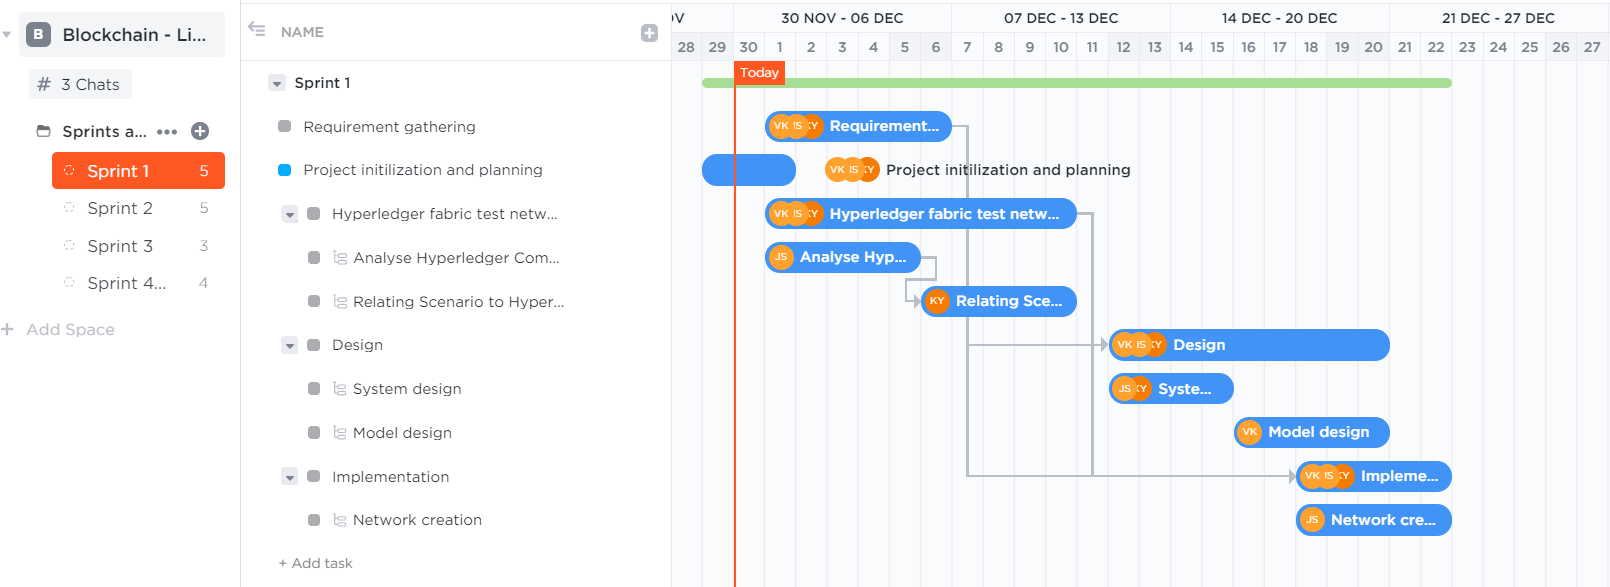
\includegraphics[width=1\textwidth]{BC_Project_Plan.png}
   
    \caption{\centering{Gantt Chart}}
    \label{fig:gantt_chart}
\end{figure}

\pagebreak

\begin{figure}[!htbp]
\centering
    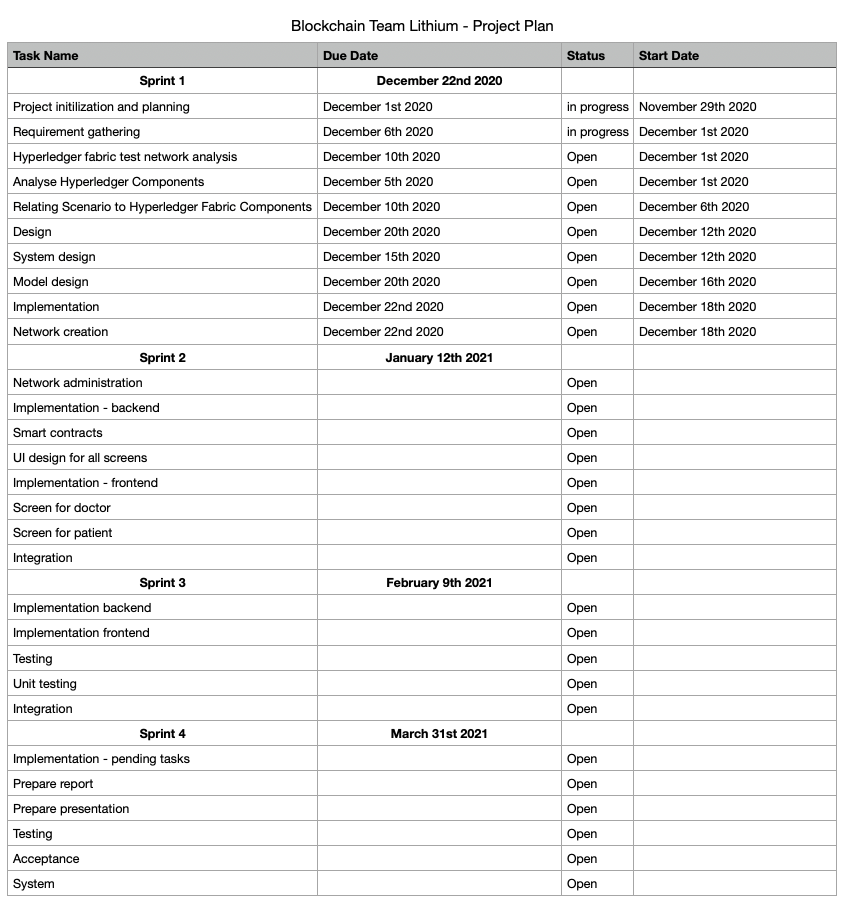
\includegraphics[width=16cm, height=18cm]{ProjectPlan.png}
    \caption{\centering{Project Plan}}
    \label{fig:projectPlan}
\end{figure}


\begin{thebibliography}{1}
\bibitem{b1} https://www.ncbi.nlm.nih.gov/pmc/articles/PMC7010942/
\bibitem{b2} https://www.ncbi.nlm.nih.gov/pmc/articles/PMC7474412/
\bibitem{b3} https://www.sciencedirect.com/science/article/pii/S2214212619306155
\bibitem{b4} https://hyperledger-fabric.readthedocs.io/ Accessed-On:01/12/2020
\bibitem{b5} https://medium.com/@lichunshen84/build-a-blockchain-poc-application-using-hyperledger-fabric-5a32687072b7, Accessed-On:01/12/2020


\end{thebibliography}



% that's all folks
\end{document}